\documentclass[conference]{IEEEtran}
\usepackage[T1]{fontenc}
\usepackage{cite,amsmath,amssymb,graphicx,xcolor,booktabs,array,tabularx,adjustbox,url,tikz}
\usetikzlibrary{positioning,arrows.meta,fit,shapes.geometric,calc}

\definecolor{trustblue}{HTML}{1F77B4}
\definecolor{trustgreen}{HTML}{2CA02C}
\definecolor{trustorange}{HTML}{FF7F0E}
\definecolor{trustred}{HTML}{D62728}
\definecolor{trustpurple}{HTML}{9467BD}

\title{ZKTrustLLM-Agents L4: n8n-Orchestrated Scientific Evaluation of Proof-Governed Agentic Zero-Trust Control for O-RAN Edge Security}

\author{
\IEEEauthorblockN{Sudarson Karmaker}
\IEEEauthorblockA{University of Surrey, 5GIC/6GIC, Guildford, United Kingdom\\
Email: s.karmaker@surrey.ac.uk}
\and
\IEEEauthorblockN{Mohammad Shojafar}
\IEEEauthorblockA{University of Surrey, 5GIC/6GIC, Guildford, United Kingdom}
}

\begin{document}
\maketitle

\begin{abstract}
Autonomous O-RAN security operations require policy-governed action, auditable evidence, replay-resistant anchoring, and reproducible evaluation. This paper presents ZKTrustLLM-Agents L4, a proof-governed agentic zero-trust framework for accountable O-RAN edge security workflows. The framework decomposes autonomy into bounded telemetry, reasoning, policy, proof, and audit/anchor agents. A self-hosted n8n workflow orchestrates scientific evaluation and generates run identifiers, Git commit binding, evidence hashes, raw logs, and paper-ready KPI tables. A clean 240-record dataset is produced across six variants, four impairment profiles, and ten repetitions per condition. Stage 3 direct runtime hooks populate anchor gas, reasoning latency, replay rejection, zero-anchor rejection, and unauthorized-submitter rejection. The result is a reviewer-verifiable evaluation method for accountable autonomous O-RAN security rather than an unconstrained agentic dashboard.
\end{abstract}

\begin{IEEEkeywords}
O-RAN, zero trust, agentic AI, n8n, zero-knowledge proof, blockchain audit, reproducible evaluation, KPI validation.
\end{IEEEkeywords}

\section{Introduction}
O-RAN disaggregates the radio access network into programmable components, including the SMO, Non-RT RIC, Near-RT RIC, rApps, and xApps. This programmability enables closed-loop optimisation but also creates security risks: unsafe autonomous action, weak evidence binding, replayed audit records, and insufficient reproducibility of security experiments.

This paper asks: \emph{how can autonomous O-RAN security actions be made policy-gated, evidence-bound, replay-resistant, and scientifically reproducible?} We answer this through ZKTrustLLM-Agents L4, a proof-governed agentic zero-trust framework.

The novelty is not the isolated use of n8n, blockchain, IPFS, or agentic AI. The novelty is their controlled scientific composition: bounded agents reason over telemetry, policy gates restrict actions, proof paths attest admissibility, audit hooks produce direct runtime evidence, and n8n orchestrates repeatable scientific evaluation. The design is motivated by zero-trust principles \cite{nist207}, O-RAN policy-control workflows \cite{oranA1}, succinct proof systems such as Groth16 \cite{groth16}, self-hosted command orchestration through n8n \cite{n8nExecute}, and the public implementation branch used for this evaluation \cite{zktrustrepo}.

\subsection{Contributions}
The paper makes five contributions: (i) a five-agent O-RAN security architecture; (ii) a policy-gated OBSERVE--REASON--PROVE--ANCHOR--ACT loop; (iii) an n8n-orchestrated evaluation pipeline; (iv) a clean 240-record dataset; and (v) Stage 3 direct runtime hooks for anchor gas, reasoning latency, replay rejection, zero-anchor rejection, and unauthorized-submitter rejection.

\section{Architecture and Threat Model}
Fig.~\ref{fig:architecture} shows the proposed architecture. The system places MNO policy at the SMO/Non-RT RIC layer and uses bounded agents for O-RAN security automation. The telemetry agent observes network and media-plane indicators. The reasoning agent maps state to trust level and candidate action. The policy agent enforces the action ladder. The proof agent supports bounded admissibility checks. The audit/anchor agent writes evidence hashes and compact commitments.

\begin{figure*}[!t]
\centering
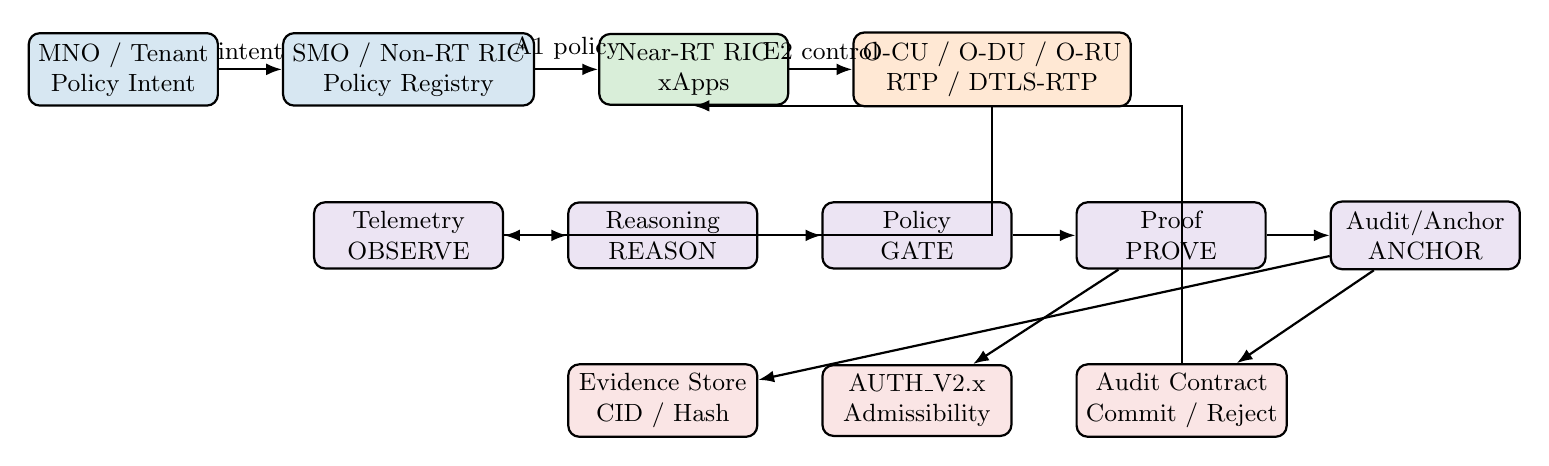
\begin{tikzpicture}[
font=\small,
box/.style={draw, rounded corners, thick, align=center, minimum height=8mm, minimum width=24mm},
arrow/.style={-{Latex[length=2mm]}, thick},
node distance=8mm
]
\node[box, fill=trustblue!18] (mno) {MNO / Tenant\\Policy Intent};
\node[box, fill=trustblue!18, right=of mno] (smo) {SMO / Non-RT RIC\\Policy Registry};
\node[box, fill=trustgreen!18, right=of smo] (nrt) {Near-RT RIC\\xApps};
\node[box, fill=trustorange!18, right=of nrt] (ran) {O-CU / O-DU / O-RU\\RTP / DTLS-RTP};

\node[box, fill=trustpurple!18, below=12mm of smo] (obs) {Telemetry\\OBSERVE};
\node[box, fill=trustpurple!18, right=of obs] (reason) {Reasoning\\REASON};
\node[box, fill=trustpurple!18, right=of reason] (policy) {Policy\\GATE};
\node[box, fill=trustpurple!18, right=of policy] (proof) {Proof\\PROVE};
\node[box, fill=trustpurple!18, right=of proof] (audit) {Audit/Anchor\\ANCHOR};

\node[box, fill=trustred!12, below=12mm of policy] (zk) {AUTH\_V2.x\\Admissibility};
\node[box, fill=trustred!12, left=of zk] (evidence) {Evidence Store\\CID / Hash};
\node[box, fill=trustred!12, right=of zk] (chain) {Audit Contract\\Commit / Reject};

\draw[arrow] (mno)--node[above]{intent}(smo);
\draw[arrow] (smo)--node[above]{A1 policy}(nrt);
\draw[arrow] (nrt)--node[above]{E2 control}(ran);
\draw[arrow] (ran.south)|-(obs.east);
\draw[arrow] (obs)--(reason);
\draw[arrow] (reason)--(policy);
\draw[arrow] (policy)--(proof);
\draw[arrow] (proof)--(audit);
\draw[arrow] (proof)--(zk);
\draw[arrow] (audit)--(evidence);
\draw[arrow] (audit)--(chain);
\draw[arrow] (chain.north)|-(nrt.south);
\end{tikzpicture}
\caption{Proposed ZKTrustLLM-Agents L4 architecture. Policy is placed in the SMO/Non-RT RIC governance path while bounded agents connect O-RAN telemetry to proof, evidence, and audit anchoring.}
\label{fig:architecture}
\end{figure*}

\begin{table}[!t]
\centering
\caption{Bounded Agentic Components}
\label{tab:agents}
\begin{adjustbox}{width=\columnwidth}
\begin{tabular}{lll}
\toprule
Agent & Role & Output \\
\midrule
Telemetry & Observe O-RAN/media KPIs & Jitter, loss, profile \\
Reasoning & Map state to trust/action & Trust state, action class \\
Policy & Enforce action ladder & Auto/Human/Privileged/Never \\
Proof & Check admissibility & AUTH\_V2.x status \\
Audit/Anchor & Bind evidence and commit & CID/hash/anchor record \\
\bottomrule
\end{tabular}
\end{adjustbox}
\end{table}


\subsection{Threat Controls}
The framework considers unapproved autonomous action, evidence tampering, anchor replay, zero/empty anchors, unsafe escalation, and unauthorized submitters. Fig.~\ref{fig:threats} maps these concepts to controls.

\begin{figure}[!t]
\centering
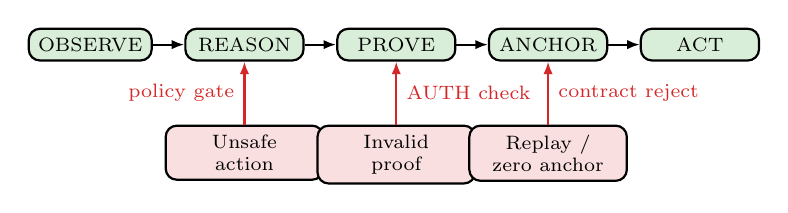
\begin{tikzpicture}[
font=\scriptsize,
phase/.style={draw, rounded corners, thick, fill=trustgreen!18, align=center, minimum width=15mm},
threat/.style={draw, rounded corners, thick, fill=trustred!15, align=center, minimum width=20mm},
arrow/.style={-{Latex[length=1.6mm]}, thick},
node distance=4mm
]
\node[phase] (o) {OBSERVE};
\node[phase, right=of o] (r) {REASON};
\node[phase, right=of r] (p) {PROVE};
\node[phase, right=of p] (a) {ANCHOR};
\node[phase, right=of a] (act) {ACT};
\draw[arrow] (o)--(r);
\draw[arrow] (r)--(p);
\draw[arrow] (p)--(a);
\draw[arrow] (a)--(act);
\node[threat, below=8mm of r] (t1) {Unsafe\\action};
\node[threat, below=8mm of p] (t2) {Invalid\\proof};
\node[threat, below=8mm of a] (t3) {Replay /\\zero anchor};
\draw[arrow, trustred] (t1)--node[left]{policy gate}(r);
\draw[arrow, trustred] (t2)--node[right]{AUTH check}(p);
\draw[arrow, trustred] (t3)--node[right]{contract reject}(a);
\end{tikzpicture}
\caption{Threat-to-control mapping. Unsafe actions are policy-gated, invalid proofs are blocked, and replay/zero anchors are rejected.}
\label{fig:threats}
\end{figure}


\subsection{Smart-Contract Boundary}
The smart contract does not control O-RAN traffic directly. Its role is trust-plane accountability: storing compact commitments, rejecting duplicate commitments, rejecting zero commitments, and enforcing authorized submitters. It cannot verify physical network truth, guarantee evidence availability, or replace MNO operational policy.

\section{Scientific Evaluation Methodology}
The evaluation is organised as a three-stage pipeline. Stage 1 establishes the n8n workflow, response matrix, KPI plan, and formal-verification preparation. Stage 2 converts outputs into a clean 240-record dataset. Stage 3 adds direct runtime hooks.

\begin{figure}[!t]
\centering
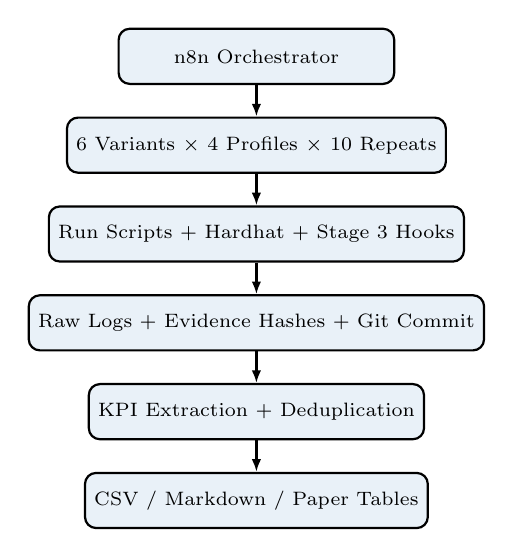
\begin{tikzpicture}[
font=\scriptsize,
box/.style={draw, rounded corners, thick, align=center, fill=trustblue!10, minimum width=35mm, minimum height=7mm},
arrow/.style={-{Latex[length=1.6mm]}, thick},
node distance=4mm
]
\node[box] (n8n) {n8n Orchestrator};
\node[box, below=of n8n] (matrix) {6 Variants $\times$ 4 Profiles $\times$ 10 Repeats};
\node[box, below=of matrix] (run) {Run Scripts + Hardhat + Stage 3 Hooks};
\node[box, below=of run] (logs) {Raw Logs + Evidence Hashes + Git Commit};
\node[box, below=of logs] (extract) {KPI Extraction + Deduplication};
\node[box, below=of extract] (paper) {CSV / Markdown / Paper Tables};
\draw[arrow] (n8n)--(matrix);
\draw[arrow] (matrix)--(run);
\draw[arrow] (run)--(logs);
\draw[arrow] (logs)--(extract);
\draw[arrow] (extract)--(paper);
\end{tikzpicture}
\caption{n8n-orchestrated scientific evaluation pipeline. n8n coordinates execution but is not a security primitive.}
\label{fig:n8n}
\end{figure}


\subsection{Evaluation Matrix}
The experiment covers six variants: Full L4, No-ZK, Oracle-only, RBAC-only, No-IPFS, and No-policy-gate. Each variant is evaluated over four impairment profiles and ten repetitions, giving 240 clean records.

\begin{table*}[!t]
\centering
\caption{Novelty and Comparison Matrix}
\label{tab:novelty}
\begin{adjustbox}{width=\textwidth}
\begin{tabular}{lccccccc}
\toprule
Approach & Agents & Policy & ZK & Evidence & Audit & Replay & KPIs \\
\midrule
O-RAN monitoring only & No & Partial & No & No & No & No & Network only \\
Blockchain logging only & No & No & No & Partial & Yes & Partial & Gas/tx \\
RBAC contract only & No & Yes & No & No & Yes & Partial & Auth/gas \\
Oracle-only trust & Yes & Weak & No & Partial & Yes & No & Score/gas \\
No-ZK ablation & Yes & Yes & No & Yes & Yes & Yes & Workflow/gas \\
Full L4 & Yes & Yes & Yes & Yes & Yes & Yes & Agent/ZK/audit \\
n8n-orchestrated L4 & Yes & Yes & Optional & Yes & Yes & Yes & 240 records \\
\bottomrule
\end{tabular}
\end{adjustbox}
\end{table*}


\subsection{KPI Classes}
The dataset distinguishes direct runtime KPIs, configured impairment-profile KPIs, and missing values. This prevents overclaiming. Configured RTP/DTLS-RTP jitter and loss values are scenario-control parameters until replaced by packet-capture or O-RAN telemetry measurements.

\subsection{Consensus-Layer Sensitivity Protocol}
The consensus mechanism belongs to the execution network, not to the Solidity contract. We therefore add a paired public-testnet protocol that deploys identical \texttt{Stage3AnomalyLedger} bytecode to Ethereum Sepolia and IoTeX testnet. Sepolia follows the Ethereum PoS protocol but uses a permissioned validator set controlled by client and testing teams \cite{ethereumNetworks}; IoTeX documents Randomized Delegated Proof of Stake (Roll-DPoS), with delegated candidate election, VRF committee selection, and PBFT voting \cite{iotexRollDpos}. IoTeX testnet is EVM compatible and uses chain ID 4690 \cite{iotexTestnet}.

Each session executes three excluded warm-up pairs and 30 measured pairs. A matched pair carries identical commitment and evidence digests, with both transactions submitted concurrently from one client host. The publication gate requires at least three sessions, verifies chain identities and runtime-code hashes, and rejects incomplete receipts, events, block samples, or security probes. The primary metric is client-observed submission-to-first-inclusion latency; it includes RPC/client overhead and public-testnet load and is not economic finality. Median confidence intervals use a two-level hierarchical bootstrap over sessions and within-session pairs. Gas prices are recorded but not converted into a cross-asset cost comparison.

\section{Results}
\subsection{KPI Completeness}
Table~\ref{tab:kpi_completeness} summarises KPI completeness after Stage 3. Anchor gas, reasoning latency, replay rejection, zero-anchor rejection, and unauthorized-submitter rejection are populated from direct runtime hooks. RTP/DTLS-RTP jitter and loss are configured impairment-profile values.

\begin{table}[!t]
\centering
\caption{KPI Completeness After Stage 3}
\label{tab:kpi_completeness}
\begin{adjustbox}{width=\columnwidth}
\begin{tabular}{lcc}
\toprule
KPI & Coverage & Evidence Type \\
\midrule
prover\_time\_ms & 160/240 & ablation/log gap \\
anchor\_gas & 240/240 & direct runtime \\
rtp\_jitter\_ms & 240/240 & configured profile \\
rtp\_loss\_pct & 240/240 & configured profile \\
reason\_latency\_ms & 240/240 & direct runtime \\
replay\_rejected & 240/240 & direct runtime \\
zero\_anchor\_rejected & 240/240 & direct runtime \\
unauthorized\_submitter & 240/240 & direct runtime \\
postAutoScore gas & 240/240 & Hardhat log \\
\bottomrule
\end{tabular}
\end{adjustbox}
\end{table}


\subsection{Variant/Profile Summary}
Table~\ref{tab:variant_summary} summarises the clean 240-record evaluation. The RBAC-only baseline was repaired to match the current contract ABI and rerun only for the affected variant, preserving experimental traceability.

\begin{table*}[!t]
\centering
\caption{Clean 240-Record Variant/Profile Summary}
\label{tab:variant_summary}
\begin{adjustbox}{width=\textwidth}
\begin{tabular}{llrrrr}
\toprule
Variant & Profile & Runs & Pass & Fail & Mean Duration (ms) \\
\midrule
full\_l4 & clean\_baseline & 10 & 10 & 0 & 39055.4 \\
full\_l4 & delay\_20ms & 10 & 10 & 0 & 47435.9 \\
full\_l4 & delay\_20ms\_jitter\_5ms & 10 & 10 & 0 & 56881.0 \\
full\_l4 & delay\_30ms\_jitter\_10ms\_loss\_1pct & 10 & 10 & 0 & 66822.6 \\
no\_ipfs & clean\_baseline & 10 & 10 & 0 & 1782.7 \\
no\_ipfs & delay\_20ms & 10 & 10 & 0 & 1742.6 \\
no\_ipfs & delay\_20ms\_jitter\_5ms & 10 & 10 & 0 & 1759.8 \\
no\_ipfs & delay\_30ms\_jitter\_10ms\_loss\_1pct & 10 & 10 & 0 & 1736.5 \\
no\_policy\_gate & clean\_baseline & 10 & 10 & 0 & 1741.3 \\
no\_policy\_gate & delay\_20ms & 10 & 10 & 0 & 1769.1 \\
no\_policy\_gate & delay\_20ms\_jitter\_5ms & 10 & 10 & 0 & 1739.7 \\
no\_policy\_gate & delay\_30ms\_jitter\_10ms\_loss\_1pct & 10 & 10 & 0 & 1743.2 \\
no\_zk & clean\_baseline & 10 & 10 & 0 & 1765.1 \\
no\_zk & delay\_20ms & 10 & 10 & 0 & 1754.2 \\
no\_zk & delay\_20ms\_jitter\_5ms & 10 & 10 & 0 & 1727.6 \\
no\_zk & delay\_30ms\_jitter\_10ms\_loss\_1pct & 10 & 10 & 0 & 1789.3 \\
oracle\_only & clean\_baseline & 10 & 10 & 0 & 1777.8 \\
oracle\_only & delay\_20ms & 10 & 10 & 0 & 1752.8 \\
oracle\_only & delay\_20ms\_jitter\_5ms & 10 & 10 & 0 & 1783.4 \\
oracle\_only & delay\_30ms\_jitter\_10ms\_loss\_1pct & 10 & 10 & 0 & 1752.5 \\
rbac\_only & clean\_baseline & 10 & 10 & 0 & 3311.4 \\
rbac\_only & delay\_20ms & 10 & 10 & 0 & 3579.0 \\
rbac\_only & delay\_20ms\_jitter\_5ms & 10 & 10 & 0 & 3606.8 \\
rbac\_only & delay\_30ms\_jitter\_10ms\_loss\_1pct & 10 & 10 & 0 & 3606.6 \\
\bottomrule
\end{tabular}
\end{adjustbox}
\end{table*}


\subsection{Stage 3 Runtime Evidence}
Stage 3 introduces an isolated Stage3AnomalyLedger micro-benchmark and a deterministic policy-reasoning probe. These emit parseable KPI lines for anchor gas, negative-security rejection, and reasoning latency.

\begin{table}[!t]
\centering
\caption{Stage 3 Direct Runtime Hook KPIs}
\label{tab:stage3}
\begin{adjustbox}{width=\columnwidth}
\begin{tabular}{lcc}
\toprule
KPI & Coverage & Result \\
\midrule
Anchor gas & 240/240 & 48961 gas \\
Reason latency & 240/240 & 4.889 ms \\
Replay rejection & 240/240 & true \\
Zero-anchor rejection & 240/240 & true \\
Unauthorized submitter & 240/240 & true \\
\bottomrule
\end{tabular}
\end{adjustbox}
\end{table}


\subsection{Multi-Model Tool-Scenario Results}
Table~\ref{tab:n8n_multimodel_tools} reports the n8n multi-model tool-scenario extension. Claude, DeepSeek, and Mistral are evaluated on evidence summarisation, claim-boundary review, and policy-ladder checking. The reported values are measured from live API calls and include JSON/schema compliance, claim-boundary agreement, action-ladder violations, and provider latency. The table is interpreted as an orchestration and bounded-reasoning robustness test, not as evidence of production O-RAN deployment, packet-capture QoE, Ethereum mainnet performance, or semantic correctness of LLM reasoning.

\begin{table*}[!t]
\centering
\caption{n8n Multi-Model Tool-Scenario Validation}
\label{tab:n8n_multimodel_tools}
\begin{adjustbox}{width=\textwidth}
\begin{tabular}{llcrrrrr}
\toprule
Provider & Model & Tool scenario & Runs & Pass (\%) & JSON (\%) & Boundary (\%) & p95 latency (ms) \\
\midrule
claude & claude-haiku-4-5-20251001 & claim-boundary-review & 10 & 0.0 & 100.0 & 100.0 & 4400.3 \\
claude & claude-haiku-4-5-20251001 & evidence-summary & 10 & 0.0 & 100.0 & 0.0 & 10287.6 \\
claude & claude-haiku-4-5-20251001 & policy-ladder-check & 10 & 0.0 & 100.0 & 100.0 & 4000.0 \\
deepseek & deepseek-chat & claim-boundary-review & 10 & 0.0 & 100.0 & 100.0 & 2498.7 \\
deepseek & deepseek-chat & evidence-summary & 10 & 0.0 & 100.0 & 0.0 & 2380.7 \\
deepseek & deepseek-chat & policy-ladder-check & 10 & 0.0 & 100.0 & 100.0 & 1653.6 \\
mistral & mistral-small-latest & claim-boundary-review & 10 & 0.0 & 100.0 & 100.0 & 1715.1 \\
mistral & mistral-small-latest & evidence-summary & 10 & 100.0 & 100.0 & 100.0 & 1536.3 \\
mistral & mistral-small-latest & policy-ladder-check & 10 & 0.0 & 100.0 & 100.0 & 941.4 \\
\bottomrule
\end{tabular}
\end{adjustbox}
\end{table*}


\section{Discussion and Limitations}
The framework intentionally avoids overclaiming. Stage3AnomalyLedger is an isolated scientific micro-benchmark, not the production trust ledger. The deterministic reasoning probe measures bounded control-plane reasoning latency, not open-ended semantic LLM reasoning. Configured impairment-profile values are not packet-capture measurements.

The main remaining direct-runtime KPI is full ZK prover timing for full-ZK rows. Current prover-time values are populated for ablation rows where the prover is intentionally not invoked, while direct prover logs are still required for full AUTH\_V2.x rows.

\section{Conclusion}
This paper presented ZKTrustLLM-Agents L4, a proof-governed and policy-gated agentic framework for accountable O-RAN edge security workflows. The contribution is a reproducible scientific evaluation pipeline that turns an autonomous dashboard into reviewer-verifiable evidence. The clean 240-record dataset, Stage 3 runtime hooks, architecture, KPI completeness report, four-family consensus comparison, local hash-primitive reference, and evidence-gated SHA-2 digest-anchoring extension provide a foundation for conference and journal-level validation without converting unmeasured protocol profiles or local execution paths into public-testnet claims.


\bibliographystyle{IEEEtran}
\bibliography{references}
\end{document}
